\documentclass[aps,reprint,superscriptaddress,11pt]{revtex4-2}
\usepackage{kotex}
\usepackage[HWP]{dhucs-interword}
\usepackage[dvips]{color}
\usepackage{graphicx}
\usepackage{bm}
\usepackage{amsmath}
\usepackage{tikz}
\usepackage{mhchem}
\usepackage{booktabs}
\usepackage{multirow}
\usepackage{array}

\begin{document}
\title{응집물질물리실험 예비보고서 \\
\small 실험주제 : Crystal Growth \& X-ray diffraction,
Structure transition of BaTiO3}

\author{HuiJae-Lee}\email{hjlee6674@inha.edu}
\affiliation{Physics Department, Inha University}

\date{\today}


\begin{abstract}
이번 실험은 X-ray diffraction을 이용하여 CaTiO$_3$, SrTiO$_3$, BaTiO$_3$를 관측하고
BaTiO$_3$의 상전이를 관측하는 것을 목적으로 한다. 각 시료들은 고상소결법을 통해 제작한다.
 \end{abstract}
 
 \maketitle
 
\section[Introduction]{Introduction}
CaTiO$_3$, SrTiO$_3$, BaTiO$_3$는 강유전성을 가진 물질이며 그 특정한 구조를 일컬어 
페로브스카이트(perovskite) 구조를 가지는 물질이다. 이런 강유전성 물질들은 현대 시대에 
축전기의 역할을 하는 물질로써 주목받고 있다. 이번 실험에서는 고상소결법을 통해 다른 물질로
부터 위 세 페로브스카이트 물질을 제조하여 X-ray diffraction으로 그 분자구조를 관찰하고
BaTiO$_3$의 유전체적 특징을 분석한다.
\section[Experiment]{Experiment}
\subsection{Theory}
\subsubsection{CaTiO$_3$, SrTiO$_3$, BaTiO$_3$}

CaTiO$_3$, SrTiO$_3$, BaTiO$_3$는 페로브스카이트 구조를 가지는 정육면체 결정의 모서리에
Ba, 면 중심에 O, 부피중심에 각각 Ca,Sr, Ti가 위치한 형태이다. 이들은 강유전성 물질이며 
고유의 퀴리온도가 존재한다. 한가지 예시로, BaTiO$_3$의 
퀴리온도는 408 K이다. 즉, $135~\mathrm{^\circ C}$ 이상의 온도로 BaTiO$_3$를 가열하면
편극이 깨진다.

\begin{figure}[htbp]
  \centering
  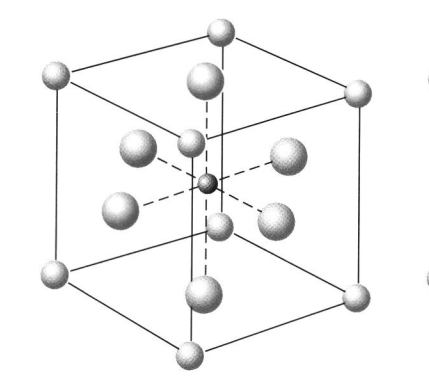
\includegraphics[scale=0.3]{BaTiO.png}
  \caption{BaTiO$_3$의 결정구조}
  \label{fig:batio}
\end{figure}

이번 실험에서 CaTiO$_3$, SrTiO$_3$, BaTiO$_3$는 각각 다음의 과정을 거쳐 합성을 진행한다.
\begin{align}
  \ce{CaCO3 + TiO2  -> CaTiO3 + CO2}  \\
  \ce{SrCO3 + TiO2  -> SrTiO3 + CO2}  \\
  \ce{BaCO3 + TiO2  -> BaTiO3 + CO2}
\end{align}
각 물질의 몰질량은 TABLE~\ref{table:1}에 적어놓았다.


\begin{table}[htp]
  \centering
  \begin{tabular}{>{\centering}p{0.2\textwidth}>{\centering\arraybackslash}p{0.2\textwidth}}
      \toprule
      Compound & molar mass (g/mol) \\
      \midrule
      \ce{BaCO3}  & 197.34 \\
      \ce{BaTiO3} & 233.19 \\
      \ce{CaCO3}  & 100.09 \\
      \ce{CaTiO3} & 135.94 \\
      \ce{SrCO3}  & 147.63 \\
      \ce{SrTiO3} & 183.49 \\
      \ce{TiO2}   & 79.866 \\
      \ce{CO2}    & 44.009 \\
      \bottomrule
  \end{tabular}
  \caption{실험에 관련된 물질들의 몰질량}\label{table:1}
\end{table}

 
\subsubsection{고상소결법}

소결은 금속 또는 세라믹 분말에 열을 가하여 밀도가 조절된 물질 또는 성분을 생산하는 공정 
기술이다. 소결은 재료과학 및 공학의 기본요소 중 합성, 가공요소로 분류되고 있다.
기본적으로 소결은 고상소결과 액상소결로 나눌 수 있다. 이번 실험에서 이용할 고상소결은
소결 온도에 도달했을 때 전체적으로 고체 상태에서 치밀화되는 과정이다. 고상소결법은 
진행 시간에 따라 크게 세 stage로 나눌 수 있는데, 순서대로 initial stage, intermediate stage,
final stage로 부른다(FIG.~\ref{fig:sintering}).

\begin{figure}[htbp]
  \centering
  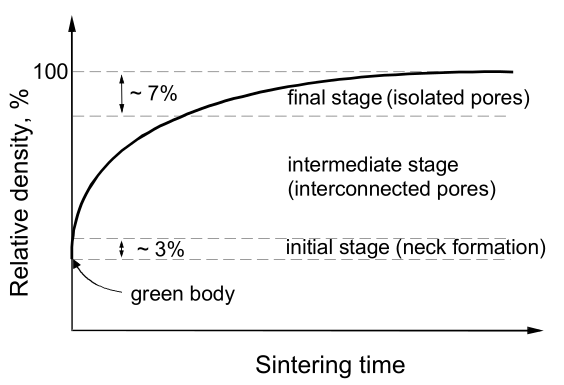
\includegraphics[scale=0.3]{sintering.png}
  \caption{고상소결 과정}\label{fig:sintering}
\end{figure}

Two-particle model에서 설명하는 initial stage는 입자 사이에 neck을 형성하는 과정이다.
neck이 형성되어 두 입자가 연결되면 물질 수송(material transport)이 일어나는데 이에 대한
많은 메카니즘이 알려져 있다(FIG.~\ref{fig:transport}).

\begin{figure}[htbp]
  \centering
  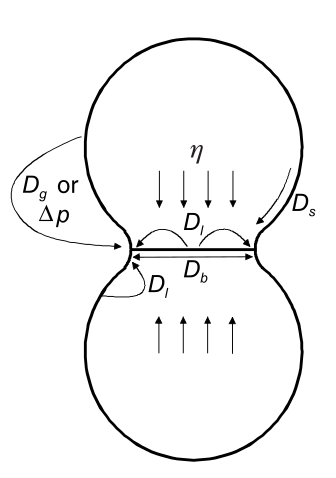
\includegraphics[scale=0.4]{transport.png}
  \caption{두 입자 사이에 형성된 neck과 물질 수송 메카니즘}\label{fig:transport}
\end{figure}

intermediate stage에서는 모든 입자의 가장자리를 따라 실린더 모양의 기공이 형성된다. 
이후 입자가 성장하면서 final stage에 도달하면 실린더 모양의 기공이 단절되고 각 꼭짓점에 
격리된 기공이 남는다(FIG.~\ref{fig:inter}). 


\begin{figure}[htbp]
  \centering
  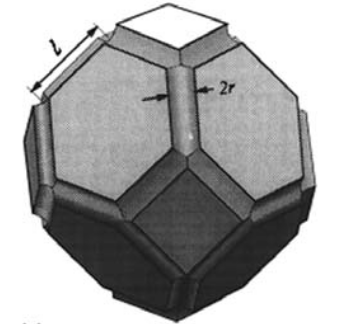
\includegraphics[scale=0.25]{intermediate.png}
  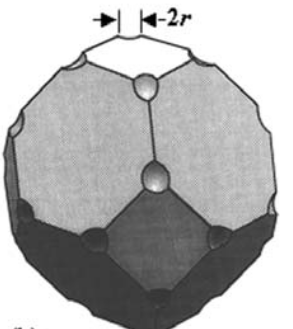
\includegraphics[scale=0.25]{final.png}
  \caption{기공이 형성된 기하학적 모델. 왼쪽부터 순서대로 intermediate stage,
  final stage에 형성되는 모델이다.}\label{fig:inter}
\end{figure}



 \subsubsection{X-ray diffraction}
X-ray diffraction는 결정 구조를 해석하는 방법 중 하나로, 브래그 법칙을 이론적인
토대로 이용한다. 결정에 X선을 입사시키면 X선의 일부는 투과하고 일부는 산란되는데
산란되는 X선은 결정 구조의 규칙성에 관한 정보를 포함한다. 규칙적으로 배열된 결정에
입사각 $\frac{\pi}{2}-\theta$로 입사하는 X선을 고려해보자(FIG~\ref{fig:bragg}).
브래그 법칙은 입사선과 평면 사이 각도 $\theta$, 결정면 사이 간격 $d$, X선의 파장 
$\lambda$ 사이 관계를 보여준다.
\begin{align}
  2d\sin{\theta} = n\lambda
\end{align}
$n$은 정수이다.

\begin{figure}[htbp]
  \centering

  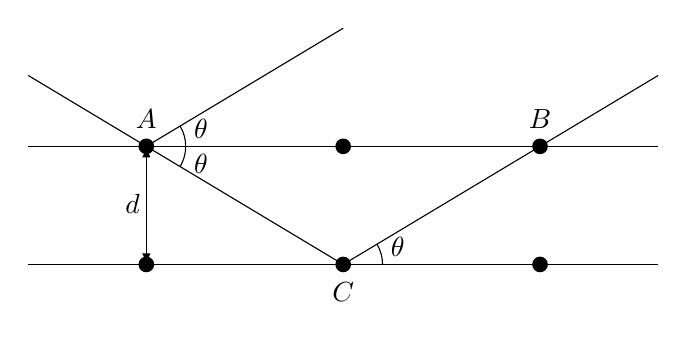
\begin{tikzpicture}
    
  \def \d {1.5}; %직선 사이 거리
  \def \x {4}; %parameter 1
  \def \y {2.5}; %점 사이 간격
  \def \t {0}; %parameter 2

  \draw (-4, \d/2) -- (4, \d/2);
  \draw (-4,-\d/2) -- (4,-\d/2);
  \draw (0,-\d/2)--(\x,  \x*\d/\y-\d/2); %C to B
  \draw (-\y,\d/2)--(\t,\d/\y*\t+3*\d/2);
  \draw (0,-\d/2)--(-\x, \x*\d/\y-\d/2); %C to A

  \node[shape=circle,fill=black,scale=0.6] at (-\y, \d/2) {};
  \draw (-\y, \d/2) node[above=3]{$A$};
  \coordinate (A) at (-\y, \d/2);
  \node[shape=circle,fill=black,scale=0.6] at ( 0, \d/2) {};
  \node[shape=circle,fill=black,scale=0.6] at ( \y, \d/2) {};
  \draw ( \y, \d/2) node[above=3]{$B$};
  \coordinate (B) at ( \y, \d/2); 
  \node[shape=circle,fill=black,scale=0.6] at (-\y,-\d/2) {};
  \node[shape=circle,fill=black,scale=0.6] at ( 0,-\d/2) {};
  \draw ( 0,-\d/2) node[below=3]{$C$};
  \coordinate (C) at ( 0,-\d/2); 
  \node[shape=circle,fill=black,scale=0.6] at ( \y,-\d/2) {};
  \draw[latex-latex] (A) -- (-\y,-\d/2) node[left=5,above=15] {$d$};
  \draw[]  (-\y+0.5, \d/2) arc(0: atan(\d/\y):0.5) 
  node[below=1,right=1.5]{$\theta$};
  \draw[]     ( 0.5,-\d/2)    arc(0: atan(\d/\y):0.5) 
  node[below=1,right=1.5]{$\theta$};
  \draw[] (-\y+0.5, \d/2) arc(0:-atan(\d/\y):0.5) 
  node[above=1,right=1.5]{$\theta$};

  \end{tikzpicture}
  \caption{결정에 입사하는 X선에 대한 브래그 법칙}
  \label{fig:bragg}
\end{figure}
\subsection{Experimental Methods}
\subsubsection{Crystal growth}
\begin{itemize}
  \item[1. ] 시료들을 중량하여 사발에 담고 막자를 이용해 30분 가량 갈아준다.
  \item[2. ] 충분히 갈아진 시료들을 캡슐에 담아 퍼니스에 넣는다.
  \item[3. ] 퍼니스에서 $800~\mathrm{^\circ C}$ 이상의 온도로 24시간 가량 시료를 가열시킨다.
  \item[4. ] 가열이 끝나면 식히기 위해 4시간 이상 대기한 후 퍼니스를 개방한다. 
  이 때 퍼니스는 개방한 상태로 2시간 더 식혀준다.
  \item[5. ] 위 2$\sim$4의 과정을 반복하여 반응하지 않은 물질이 없도록 한다. 
\end{itemize}
\subsubsection{X-ray diffraction}
\begin{itemize}
  \item[1. ] 제작된 시료를 인하대학교 표준분석연구원에 의뢰한다. 예약은 일주일 전에 미리 
  하도록 한다.
  \item[2. ] 측정 데이터를 분석한다.
\end{itemize}
\subsubsection{Structure transition of \ce{BaTiO3} }
\begin{itemize}
  \item[1. ] 여분의 \ce{BaTiO3}를 이용하여 다음 과정을 따라 펠릿을 제작한다.
  \begin{itemize}
    \item [(1)] \ce{BaTiO3}가루를 펠릿 틀 안에 넣고 공기를 빼서 평평하게 편다.
    \item [(2)] 펠릿 틀을 유압프레스에 넣어 1 t의 무게로 압축한다.
    \item [(3)] 30분 가량 압축 후 퍼니스에서 가열한다.
  \end{itemize}
  \item[2. ] 에나멜선의 한쪽 피복을 제거해 펠릿에 위치시키고 sliver paste를 바른 후 30분 이상 건조시킨다.
  \item[3. ] sliver paste 위에 silver epoxy를 넘치지 않도록 바른다.
  \item[4. ] sliver가 굳도록 $100~\mathrm{^\circ C}$ 이상의 온도로 30분 이상 가열시킨다.
  \item[5. ] 펠릿에 뒷면에도 같은 방법으로 에나멜선을 연결한다.
  \item[6. ] 핫플레이트 위에 실리콘 액체가 담긴 비커를 두고 온도계를 바닥에서 띄워서 고정시킨다.
  \item[7. ] 에나멜선을 LCR미터에 연결하여 온도에 따른 캐패시턴스와 전기변위장을 측정한다.
  \item[8. ] 다른 진동수 값에서도 실험을 반복하고 USB를 이용해 데이터를 추출한다.
\end{itemize}
\nocite{*} 
\bibliography{ref}



%\begin{thebibliography}{9}
%\end{thebibliography}

\vfill
\end{document}